\chapter{Geração de cenários por Monte Carlo}
\label{cap:cenarios}

O objetivo desta etapa é construir um conjunto representativo de configurações operacionais da rede IEEE~34 barras sob diferentes condições de inserção de geração fotovoltaica e de BESS, permitindo a avaliação probabilística do impacto desses recursos sobre os perfis de tensão. As configurações incluem o nível de penetração FV, a distribuição espacial e o dimensionamento das unidades FV e BESS, o tipo de dia e o respectivo perfil de irradiância, e o perfil de carga da rede.

\section{O método de Monte Carlo}
\label{sec:montecarlo}

A simulação de Monte Carlo é uma técnica numérica que, em contraste com abordagens determinísticas, incorpora explicitamente as incertezas do sistema por meio de distribuições de probabilidade. Cada variável é associada à sua distribuição; para cada cenário, os valores são sorteados aleatoriamente e empregados na execução do modelo. Repetindo-se o procedimento um número elevado de vezes, obtém-se não um único resultado determinístico, mas uma distribuição de comportamentos possíveis, a partir da qual se calculam estatísticas descritivas --- média, desvio padrão, percentis e probabilidade de violação de limites.

Para a avaliação do impacto de cada cenário sobre os perfis de tensão ao longo de um dia, emprega-se a simulação de fluxo de potência quasi-estática~\cite{cunha2021}, executada em patamares horários ao longo das 24~horas, capturando a variação temporal da geração FV e da demanda. O procedimento se organiza em três etapas: (i)~geração dos cenários pelo método de Monte Carlo, sorteando combinações de localização e potência dos sistemas FV, capacidade dos BESS e perfis de irradiância e carga; (ii)~simulação do fluxo de potência de cada cenário no OpenDSS, extraindo os perfis de tensão de todas as barras; e (iii)~análise estatística dos resultados, consolidados por nível de penetração.

As variáveis estocásticas dividem-se em quatro grupos: a alocação e o dimensionamento das unidades FV; a alocação e o dimensionamento das unidades BESS; o perfil de irradiância solar; e os fatores de incerteza aplicados aos perfis de carga. O nível de penetração fotovoltaica, $\eta$, é definido como a razão entre a potência nominal total instalada dos sistemas FV e a demanda de pico total da rede. Foram considerados onze níveis, de 0\% a 100\% em incrementos de 10\%, com 500~cenários independentes por nível, totalizando 5500~cenários simulados.

\section{Alocação e dimensionamento dos sistemas FV}
\label{sec:alocacao_fv}

Os sistemas FV foram restritos às barras que alimentam cargas trifásicas do alimentador (barras 860, 840, 844, 848 e 890), evitando o desequilíbrio que uma injeção monofásica de grande magnitude introduziria na rede. A potência nominal total dos sistemas FV de cada cenário é determinada diretamente pelo nível de penetração $\eta$ e pela demanda de pico $P_\text{pico} = 1{,}769$~MW, conforme a Equação~\eqref{eq:pfv_total}:
\begin{equation}
  P_\text{FV}^\text{total} = P_\text{pico}\,\eta.
  \label{eq:pfv_total}
\end{equation}

A distribuição de $P_\text{FV}^\text{total}$ entre as barras segue uma alocação proporcional com perturbação gaussiana controlada, adotada para evitar que a variabilidade espacial domine a variância dos resultados de tensão. Cada uma das $N=5$ barras trifásicas elegíveis recebe uma fração $w_j$ da potência total, obtida pela normalização de um fator multiplicativo $g_j$ sorteado de forma independente, segundo as Equações~\eqref{eq:fv_aloc}:
\begin{subequations}
  \label{eq:fv_aloc}
  \begin{align}
    g_j &\sim \mathcal{N}(1{,}0,\ \sigma_\text{aloc}^2), \qquad g_j \in [0{,}5;\ 1{,}5], \label{eq:fv_g}\\
    w_j &= \frac{g_j}{\sum_{k=1}^{N} g_k}, \label{eq:fv_w}\\
    P_{\text{FV},j} &= P_\text{FV}^\text{total}\, w_j. \label{eq:fv_pj}
  \end{align}
\end{subequations}
O fator $g_j$ é truncado ao intervalo $[0{,}5;\ 1{,}5]$, de modo que nenhuma barra receba menos de 0,5 nem mais de 1,5 vez a fração média; a variância $\sigma_\text{aloc}^2$ controla a dispersão espacial da potência FV. A normalização em~\eqref{eq:fv_w} garante que os pesos somem a unidade, redistribuindo a potência total sem alterar o montante instalado.

\section{Alocação e operação dos BESS}
\label{sec:alocacao_bess}

Assim como os sistemas FV, as unidades BESS foram restritas às barras trifásicas. A potência nominal total do conjunto de BESS é fixada como fração de 35\% da potência FV total instalada, conforme a Equação~\eqref{eq:bess_total}:
\begin{equation}
  P_\text{BESS}^\text{total} = 0{,}35\, P_\text{FV}^\text{total}.
  \label{eq:bess_total}
\end{equation}
Essa regra garante que a capacidade de armazenamento cresça proporcionalmente à geração FV instalada, coerente com o objetivo dos BESS de absorver o excedente diurno e fornecer energia no pico noturno. A potência $P_\text{BESS}^\text{total}$ é distribuída entre as cinco barras trifásicas pelo mesmo mecanismo proporcional com perturbação gaussiana adotado para a alocação FV, com $\sigma_\text{BESS} = 0{,}10$.

Nesta etapa, o modelo de fluxo de potência não rastreia o estado de carga das baterias ao longo do tempo: o BESS é tratado como uma fonte ou carga de potência controlada, com perfil de operação determinístico e idêntico para todos os cenários e níveis de penetração. Esse perfil, $b(h)$, é definido pela Equação~\eqref{eq:bess_perfil}:
\begin{equation}
  b(h) =
  \begin{cases}
    -1{,}0, & h \in [10,\ 14] \quad \text{(carregamento)},\\
    +1{,}0, & h \in [18,\ 21] \quad \text{(descarregamento)},\\
    0{,}0,  & \text{caso contrário},
  \end{cases}
  \label{eq:bess_perfil}
\end{equation}
de modo que a potência efetiva absorvida ou injetada pela unidade da barra $j$ na hora $h$ é $P_{\text{BESS},j}(h) = P_{\text{BESS},j}\, b(h)$. A Figura~\ref{fig:perfil_bess} ilustra a curva de carregamento e descarregamento. Trata-se de uma simplificação desta etapa; um despacho otimizado em tempo real é objeto das etapas subsequentes do projeto.

\begin{figure}[!htb]
  \centering
  \caption{Curva de carregamento e descarregamento das unidades BESS.}
  \label{fig:perfil_bess}
  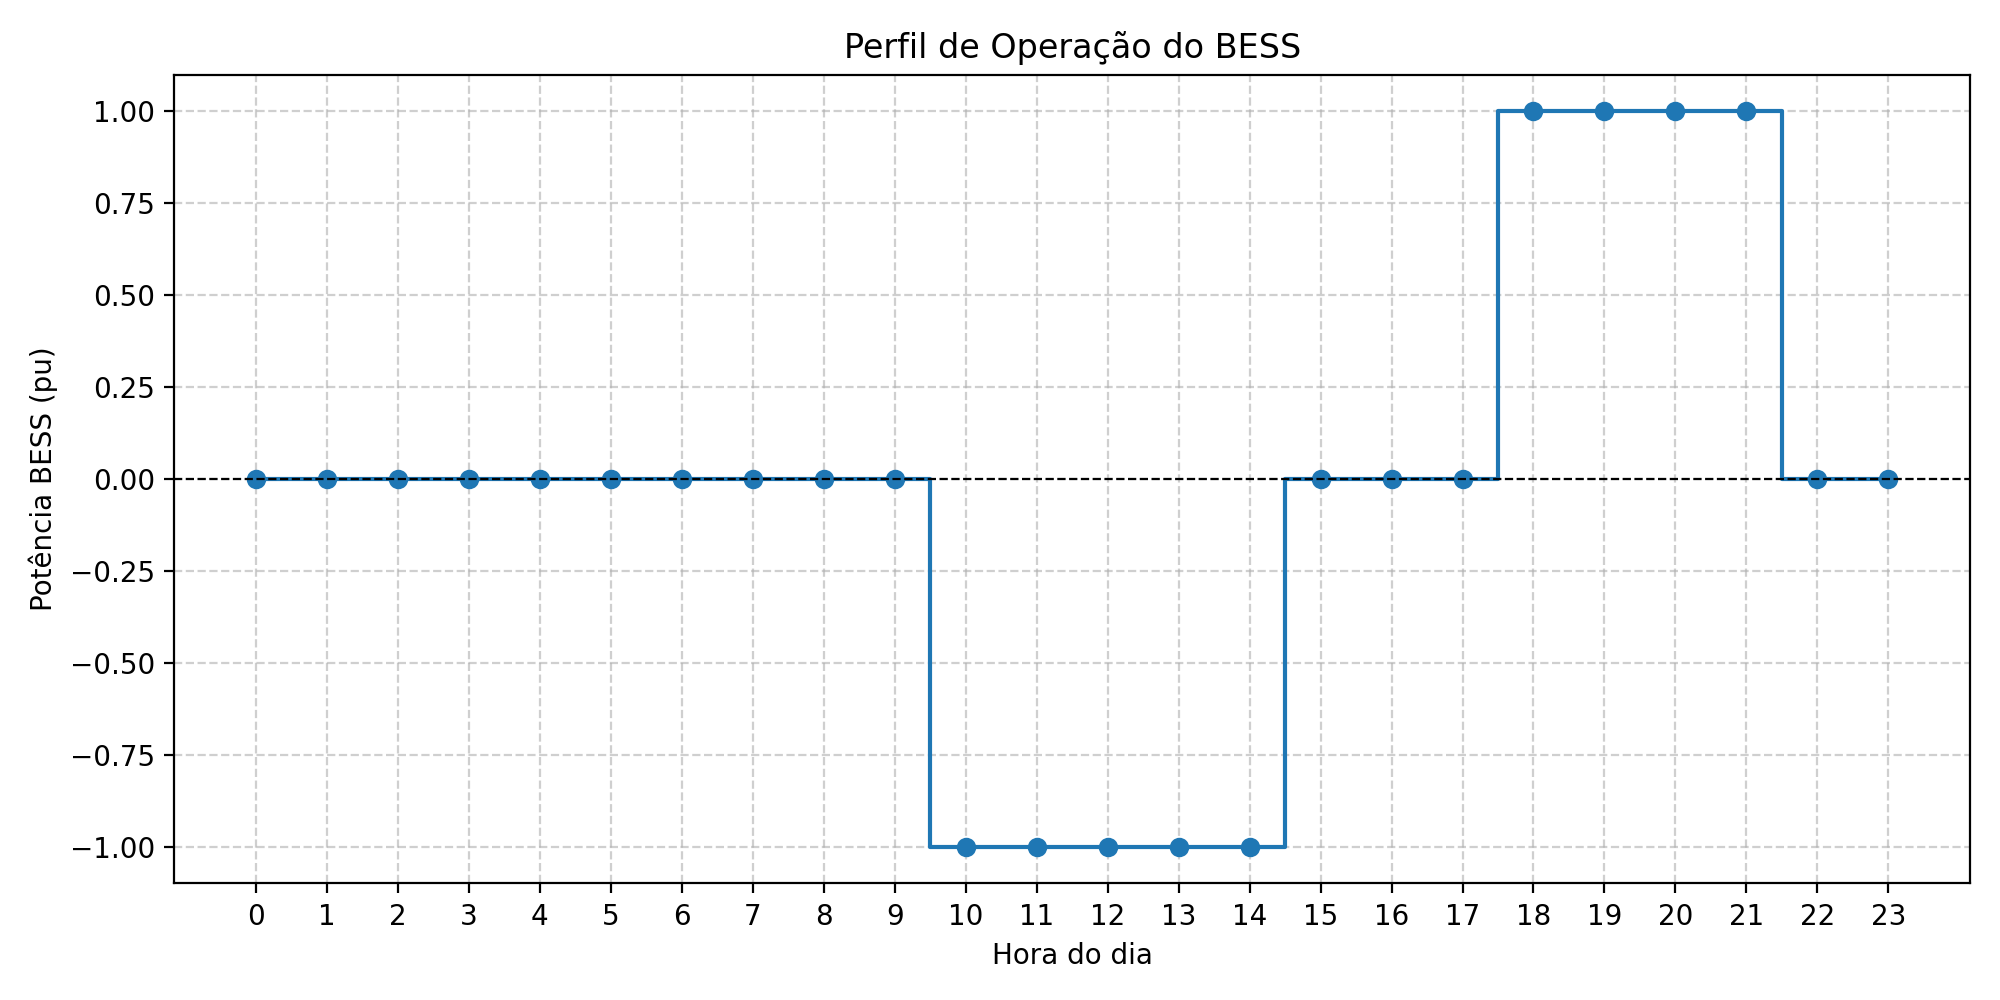
\includegraphics[width=0.72\textwidth]{perfil_bess.png}
  \par\vspace{2pt}\fonte{autoria própria}
\end{figure}

\section{Dia típico e perfil de irradiância}
\label{sec:irradiancia}

Para a geração dos perfis de irradiância, adotou-se um padrão misto que combina a categorização de dias típicos com o acréscimo de ruído gaussiano. A base de dados é proveniente do Sistema de Organização Nacional de Dados Ambientais (SONDA), operado pelo INPE~\cite{inpe_sonda}; utilizaram-se medições da estação de Cachoeira Paulista (SP) entre janeiro de 2023 e dezembro de 2025, tratadas para a remoção de valores espúrios e de dias incompletos.

A modelagem de dias típicos baseia-se no índice de claridade, definido na Equação~\eqref{eq:kt} como a razão entre a irradiância global horizontal integrada diariamente na superfície ($H$) e a irradiância extraterrestre teórica para o mesmo dia e local ($H_0$)~\cite{lai2017}:
\begin{equation}
  k_t = \frac{H}{H_0}.
  \label{eq:kt}
\end{equation}
Com base em $k_t$, definiram-se três dias típicos --- Céu Aberto, Parcialmente Nublado e Nublado ---, conforme a Tabela~\ref{tab:dias_tipicos}. A frequência de ocorrência de cada classe no período analisado (Figura~\ref{fig:kt}) foi utilizada como probabilidade no sorteio do tipo de dia em cada cenário.

\begin{table}[!htb]
  \centering
  \caption{Classificação dos dias típicos com base no índice de claridade $k_t$.}
  \label{tab:dias_tipicos}
  \begin{tabular}{@{}ll@{}}
    \toprule
    \textbf{Dia típico} & \textbf{Índice de claridade} \\
    \midrule
    Céu Aberto            & $k_t > 0{,}6$ \\
    Parcialmente Nublado  & $0{,}3 < k_t < 0{,}6$ \\
    Nublado               & $k_t < 0{,}3$ \\
    \bottomrule
  \end{tabular}
  \par\vspace{2pt}\fonte{autoria própria}
\end{table}

\begin{figure}[!htb]
  \centering
  \caption{Distribuição do índice de claridade no período analisado.}
  \label{fig:kt}
  
\includegraphics[width=0.7\textwidth]{sonda_classificacao_kt.png}
  \par\vspace{2pt}\fonte{autoria própria}
\end{figure}

Para cada dia típico, obteve-se a curva de irradiância diária por hora, normalizada pelo respectivo valor máximo para eliminar o efeito da variação sazonal (Figura~\ref{fig:perfis_irradiancia}). O perfil de céu aberto apresenta curva simétrica, com máximo próximo de 0,98~p.u. ao meio-dia solar; o parcialmente nublado é semelhante em forma, com amplitude ligeiramente menor; e o nublado exibe valores significativamente menores e distribuição mais achatada.

\begin{figure}[!htb]
  \centering
  \caption{Perfis horários típicos de irradiância normalizada.}
  \label{fig:perfis_irradiancia}
  
\includegraphics[width=0.7\textwidth]{sonda_perfis_irradiancia.png}
  \par\vspace{2pt}\fonte{autoria própria}
\end{figure}

Uma vez sorteado o tipo de dia, o perfil de irradiância do cenário $s$ é gerado introduzindo um ruído multiplicativo gaussiano hora a hora sobre o perfil médio correspondente, $\bar{I}(h)$, conforme a Equação~\eqref{eq:irradiancia}:
\begin{equation}
  I_s(h) = \operatorname{clip}\!\big[\,\bar{I}(h)\,(1 + \varepsilon(h)),\ 0,\ 1\,\big], \qquad \varepsilon(h) \sim \mathcal{N}(0,\ \sigma_i^2),
  \label{eq:irradiancia}
\end{equation}
em que $\varepsilon(h)$ é um ruído independente para cada hora, com desvio padrão relativo $\sigma_i$ inversamente proporcional ao índice de claridade --- quanto menor a claridade, maior a variabilidade ---, e a operação $\operatorname{clip}$ mantém o fator no intervalo fisicamente admissível $[0,\ 1]$. O mesmo perfil $I_s(h)$ é aplicado a todas as unidades FV de um dado cenário, hipótese de correlação espacial perfeita razoável para a extensão limitada da rede. A potência injetada por uma unidade de potência nominal $P_\text{FV}$ na hora $h$ é, portanto, $P_{\text{FV},s}(h) = P_\text{FV}\, I_s(h)$.

\section{Perfil de carga estocástico}
\label{sec:carga_estocastica}

Sobre os perfis de carga determinísticos descritos na Seção~\ref{sec:perfis_carga}, sobrepõe-se, em cada cenário, uma variabilidade estocástica. Para cada uma das barras de carga sorteia-se um fator multiplicativo $f_b$ a partir de uma distribuição normal de desvio padrão relativo $\sigma_d = 0{,}1$, truncado ao intervalo $[0{,}80;\ 1{,}20]$, conforme a Equação~\eqref{eq:carga}:
\begin{equation}
  f_b \sim \mathcal{N}(1{,}0,\ \sigma_d^2), \qquad f_b \in [0{,}80;\ 1{,}20].
  \label{eq:carga}
\end{equation}
Esse fator, mantido constante ao longo do dia para cada barra, representa a heterogeneidade entre consumidores. A potência efetiva na barra $b$ na hora $h$ resulta de $P_b(h) = P_b^\text{nom}\, f_b\, c(h)$, em que $P_b^\text{nom}$ é a potência nominal da barra e $c(h)$ o respectivo perfil de carga horário. Os fatores são sorteados de forma independente entre barras, o que implica ausência de correlação espacial na incerteza de demanda --- simplificação conservadora justificada pelo objetivo de gerar cenários-base para a avaliação do impacto da penetração FV.
